
\coverchapter{Results}\label{ch:results}
\section{Cross domain successes}
The search method we have developed and the resulting bijection works between different domains. The problem however is the lack of maintained implementations of domains using \css{}. With \css{} being a product of a research group that is mainly interested in permutation patterns, unsurprisingly the most supported domain is \tsc{}.

There is a very simple example for words provided in the project's repository. A word over an alphabet $\Sigma$ is any sequence of elements from $\Sigma$. A pattern in words is another word that occurs as a subsequence. This class can be described as a triple $\mathcal{W} = (p, \Sigma, A)$, where $p$ is a required prefix, $\Sigma$ is the alphabet and $A$ is the set of patterns to avoid. For example $(\varepsilon, \set{0,1}, \set{11})$ is the set of binary strings that avoid consecutive ones, that is
\[
    (\varepsilon, \set{0,1}, \set{11}) = \set{\varepsilon, 0, 1, 00, 01, 10, 000, 001, 010, 100, 101, \dotsc}.
\]


The bijection search will easily find bijections between sets such as $(\varepsilon, \set{0,1}, \set{11})$ and $(\varepsilon, \set{a,b}, \set{bb})$, that are identical given a mapping of the letters of the alphabet. The same goes for the trivial sets $(\epsilon, \set{0}, \emptyset)$ and $\Av{12}$, where there is only a single element of each length. The implementation for words has few strategies and limited effort was allocated to finding bijections between words and permutation classes. We will demonstrate two such bijections in greater detail but there is a caveat that needs to be addressed.

Take the class $\mathcal{W} = (\varepsilon, \set{a,b}, \emptyset)$ for example. For any fixed length $n$, there are $2^n$ unique words as we have a choice between two letters for each position in any sequence. This produces the sequence 
\[
    1, 2, 4, 8, 16, 32, 64, \dotsc
\]
while the permutation class, $\Av{231,321}$, has the sequence 
\[
    1, 1, 2, 4, 8, 16, 32, \dotsc
\]
which is off by one. We could use $\textsf{Av}_{\geq1}(231,312)$ instead, which shares this sequence with the words, but that brings another problem. Words of length $n$ would map to permutations of length $n+1$ while parallel specifications requires atoms to match. What we can do instead, is placing the largest point of $\textsf{Av}_{\geq1}(231,312)$ and factoring it out. That leaves us with a tiling root $\mathcal{T}$ where
\begin{align*}
    \Av{231,312} &\cong \set{\varepsilon} \sqcup \textsf{Av}_{\geq1}(231,312),\\
    \textsf{Av}_{\geq1}(231,312) &\cong \set{\point{0.1}}\times \textsf{Grid}(\mathcal{T}).
\end{align*}
The tiling in question here is
\[
    \mathcal{T} = \left((2,1), \set{2^{(0,0)}1^{(1,0)}, 21^{(1,0)}, 231^{(0,0)}, 321^{(0,0)}},\emptyset\right).
\]
Now we can find and construct bijections between $\mathcal{W}$ and $\textsf{Grid}(\mathcal{T})$. This will map the words to gridded permutations in $\mathcal{G}^{(2,1)}$ instead of $\mathcal{G}^{(1,1)}$, but the mapping from them to permutations is trivial.

The other bijection found was between $\mathcal{W} = (\varepsilon, \set{0,1}, \set{11})$ and $\Av{231,312,321}$. These are counted by the Fibonacci numbers but here we have the same issue as before, with one sequence being off my one. We remedy this exactly the same way as before, leaving us with a tiling root that can be seen in figure \FigureRef{fig:fibpermoffbyone}. This tiling can have at most a single point in cell $(1,0)$ and if it includes one, it must be greater than all the points in cell $(0,0)$. This can easily by mapped back to permutation by appending $n+1$ to the underlying permutation for any gridded permutation that has no points in cell $(1,0)$ and for those that do, we place $n+1$ immediately prior to the last element. \TableRef{tab:wordtilmap} shows the bijection constructed for $n \in \set{0,1,2,3}$ and the corresponding permutation with the mapping described above. 

\begin{figure}[ht!]
    \centering
    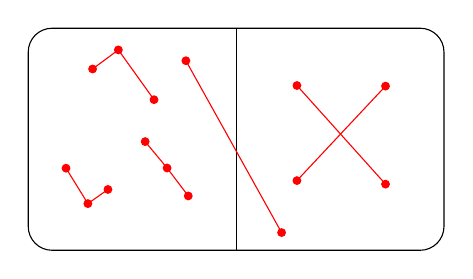
\begin{tikzpicture}[scale=1, every node/.style={scale=1}]
    \def\xscale{0.75} % Horizontal scale factor
    \def\yscale{0.75} % Vertical scale factor
    \def\spnt{0.075*0.75} % Size of smaller points
    \def\lpnt{0.125*0.75} % Size of larger points
    \draw (3.52*\xscale, 3.76*\yscale) -- (3.52*\xscale, 0);
    \draw[rounded corners=2ex] (0,0) rectangle (7.04*\xscale,3.76*\yscale);
    
    \fill[red] (4.55*\xscale, 1.18*\yscale) circle (\spnt);
    \fill[red] (6.05*\xscale, 2.78*\yscale) circle (\spnt);
    \draw[red] (4.55*\xscale, 1.18*\yscale) -- (6.05*\xscale,2.78*\yscale);
    
    \fill[red] (4.55*\xscale, 2.79*\yscale) circle (\spnt);
    \fill[red] (6.05*\xscale, 1.12*\yscale) circle (\spnt);
    \draw[red] (4.55*\xscale, 2.79*\yscale) -- (6.05*\xscale,1.12*\yscale);
    
    \fill[red] (2.67*\xscale, 3.21*\yscale) circle (\spnt);
    \fill[red] (4.29*\xscale, 0.3*\yscale) circle (\spnt);
    \draw[red] (2.67*\xscale, 3.21*\yscale) -- (4.29*\xscale,0.3*\yscale);
    
    \fill[red] (1.09*\xscale, 3.07*\yscale) circle (\spnt);
    \fill[red] (1.526001050877835*\xscale, 3.393088634545991*\yscale) circle (\spnt);
    \fill[red] (2.13*\xscale, 2.55*\yscale) circle (\spnt);
    \draw[red] (1.09*\xscale, 3.07*\yscale) -- (1.526001050877835*\xscale,3.393088634545991*\yscale) -- (2.13*\xscale,2.55*\yscale);
    
    \fill[red] (0.64*\xscale, 1.39*\yscale) circle (\spnt);
    \fill[red] (1.01*\xscale, 0.79*\yscale) circle (\spnt);
    \fill[red] (1.35*\xscale, 1.03*\yscale) circle (\spnt);
    \draw[red] (0.64*\xscale, 1.39*\yscale) -- (1.01*\xscale,0.79*\yscale) -- (1.35*\xscale,1.03*\yscale);
    
    \fill[red] (1.98*\xscale, 1.84*\yscale) circle (\spnt);
    \fill[red] (2.3511520552717013*\xscale, 1.3932029657051672*\yscale) circle (\spnt);
    \fill[red] (2.71*\xscale, 0.92*\yscale) circle (\spnt);
    \draw[red] (1.98*\xscale, 1.84*\yscale) -- (2.3511520552717013*\xscale,1.3932029657051672*\yscale) -- (2.71*\xscale,0.92*\yscale);
\end{tikzpicture}
    \caption{The tiling required to deal with off by one and atom matching to find a bijection between binary strings with no consecutive ones and $\Av{231,312,321}$.}
    \label{fig:fibpermoffbyone}
\end{figure}

\begin{table}[ht!]
    \centering
    \begin{tabular}{c|c|c}
        Word & Gridded permutation & Permutation\\
        \hline
        $\varepsilon$ & $\varepsilon$ & $1$\\
        $0$ & $1^{(0,0)}$ & $12$\\
        $1$ & $1^{(1,0)}$ & $21$\\
        $00$ & $12^{(0,0)}$ & $123$\\
        $01$ & $21^{(0,0)}$ & $213$\\
        $10$ & $1^{(0,0)}2^{(1,0)}$ & $132$\\
        $000$ & $123^{(0,0)}$ & $1234$\\
        $001$ & $213^{(0,0)}$ & $2134$\\
        $010$ & $132^{(0,0)}$ & $1324$\\
        $100$ & $12^{(0,0)}3^{(1,0)}$ & $1243$\\
        $101$ & $21^{(0,0)}3^{(1,0)}$ & $2143$\\
    \end{tabular}
    \caption{An automated bijection between binary strings avoiding consecutive ones and a slightly altered tiling for $\Av{231,312,321}$ and the permutation corresponding to each gridded permutation.}
    \label{tab:wordtilmap}
\end{table}




\begin{figure}
    \centering
    % TODO: Redo this crap properly 

{
\newcommand{\wordclass}[2]{%
\begin{tikzpicture}[scale=0.3, baseline=(current bounding box.center)]
\useasboundingbox (0,-3) rectangle (#1,3);
			\draw[thick, rounded corners=3pt] (0,0) rectangle (#1,3);
			\node at ({#1/2}, 1.5) {#2};
;
			    \end{tikzpicture}
}

\newcommand{\tnodeempty}{%
\begin{tikzpicture}[scale=0.3, baseline=(current bounding box.center)]
\useasboundingbox (0,-3) rectangle (3,3);
			\draw[thick, rounded corners=3pt] (0,0) rectangle (3,3);
			\draw[pattern=north west lines, pattern color=lightgray]  (3,0) to[rounded corners=3pt] (0,0) to[rounded corners=3pt] (0,3) to[rounded corners=3pt] (3,3) to[rounded corners=3pt] cycle;
;
			    \end{tikzpicture}
}

\newcommand{\todesingle}[1]{%
\begin{tikzpicture}[scale=0.3, baseline=(current bounding box.center)]
\useasboundingbox (0,-3) rectangle (3,3);
			\draw[thick, rounded corners=3pt] (0,0) rectangle (3,3);
			\node at (1.5, 1.5) {#1};
;
			    \end{tikzpicture}
}
\newcommand{\tone}{%
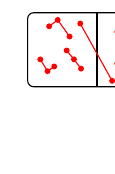
\begin{tikzpicture}[scale=0.25, every node/.style={scale=0.25}, baseline=(current bounding box.center)]
\useasboundingbox (0,-3) rectangle (3,3);
\def\xscale{1} % Horizontal scale factor
\def\yscale{1} % Vertical scale factor
\def\spnt{0.15} % Size of smaller points
\def\lpnt{0.125} % Size of larger points
\draw (3.52*\xscale, 3.76*\yscale) -- (3.52*\xscale, 0);
\draw[rounded corners=2ex*0.25] (0,0) rectangle (7.04*\xscale,3.76*\yscale);
\fill[red] (4.55*\xscale, 1.18*\yscale) circle (\spnt);
\fill[red] (6.05*\xscale, 2.78*\yscale) circle (\spnt);
\draw[red] (4.55*\xscale, 1.18*\yscale) -- (6.05*\xscale,2.78*\yscale);
\fill[red] (4.55*\xscale, 2.79*\yscale) circle (\spnt);
\fill[red] (6.05*\xscale, 1.12*\yscale) circle (\spnt);
\draw[red] (4.55*\xscale, 2.79*\yscale) -- (6.05*\xscale,1.12*\yscale);
\fill[red] (2.67*\xscale, 3.21*\yscale) circle (\spnt);
\fill[red] (4.29*\xscale, 0.3*\yscale) circle (\spnt);
\draw[red] (2.67*\xscale, 3.21*\yscale) -- (4.29*\xscale,0.3*\yscale);
\fill[red] (1.09*\xscale, 3.07*\yscale) circle (\spnt);
\fill[red] (1.526001050877835*\xscale, 3.393088634545991*\yscale) circle (\spnt);
\fill[red] (2.13*\xscale, 2.55*\yscale) circle (\spnt);
\draw[red] (1.09*\xscale, 3.07*\yscale) -- (1.526001050877835*\xscale,3.393088634545991*\yscale) -- (2.13*\xscale,2.55*\yscale);
\fill[red] (0.64*\xscale, 1.39*\yscale) circle (\spnt);
\fill[red] (1.01*\xscale, 0.79*\yscale) circle (\spnt);
\fill[red] (1.35*\xscale, 1.03*\yscale) circle (\spnt);
\draw[red] (0.64*\xscale, 1.39*\yscale) -- (1.01*\xscale,0.79*\yscale) -- (1.35*\xscale,1.03*\yscale);
\fill[red] (1.98*\xscale, 1.84*\yscale) circle (\spnt);
\fill[red] (2.3511520552717013*\xscale, 1.3932029657051672*\yscale) circle (\spnt);
\fill[red] (2.71*\xscale, 0.92*\yscale) circle (\spnt);
\draw[red] (1.98*\xscale, 1.84*\yscale) -- (2.3511520552717013*\xscale,1.3932029657051672*\yscale) -- (2.71*\xscale,0.92*\yscale);
\end{tikzpicture} 
}
\newcommand{\ttwo}{%
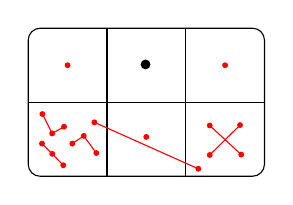
\begin{tikzpicture}[scale=0.5, every node/.style={scale=0.5}]
\def\xscale{1.0} % Horizontal scale factor
\def\yscale{1.0} % Vertical scale factor
\def\spnt{0.075} % Size of smaller points
\def\lpnt{0.125} % Size of larger points
\draw[rounded corners=2ex*0.5] (0,0) rectangle (6*\xscale,3.76*\yscale);
\draw (2.0*\xscale, 3.76*\yscale) -- (2.0*\xscale, 0);
\draw (4.0*\xscale, 3.76*\yscale) -- (4.0*\xscale, 0);
\draw (0, 1.88*\yscale) -- (6.0*\xscale, 1.88*\yscale);
\fill[red] (4.61*\xscale, 0.54*\yscale) circle (\spnt);
\fill[red] (5.38*\xscale, 1.3*\yscale) circle (\spnt);
\draw[red] (4.61*\xscale, 0.54*\yscale) -- (5.38*\xscale,1.3*\yscale);
\fill[red] (1.68*\xscale, 1.37*\yscale) circle (\spnt);
\fill[red] (4.32*\xscale, 0.19*\yscale) circle (\spnt);
\draw[red] (1.68*\xscale, 1.37*\yscale) -- (4.32*\xscale,0.19*\yscale);
\fill[red] (4.61*\xscale, 1.29*\yscale) circle (\spnt);
\fill[red] (5.41*\xscale, 0.55*\yscale) circle (\spnt);
\draw[red] (4.61*\xscale, 1.29*\yscale) -- (5.41*\xscale,0.55*\yscale);
\fill[red] (1.12*\xscale, 0.83*\yscale) circle (\spnt);
\fill[red] (1.4096601986560762*\xscale, 1.0249991174784614*\yscale) circle (\spnt);
\fill[red] (1.73*\xscale, 0.59*\yscale) circle (\spnt);
\draw[red] (1.12*\xscale, 0.83*\yscale) -- (1.4096601986560762*\xscale,1.0249991174784614*\yscale) -- (1.73*\xscale,0.59*\yscale);
\fill[red] (1*\xscale, 2.82*\yscale) circle (\spnt);
\fill[red] (5*\xscale, 2.82*\yscale) circle (\spnt);
\fill[red] (3*\xscale, 1*\yscale) circle (\spnt);
\fill[red] (0.36*\xscale, 1.58*\yscale) circle (\spnt);
\fill[red] (0.6091281492290661*\xscale, 1.0877096738635244*\yscale) circle (\spnt);
\fill[red] (0.91*\xscale, 1.26*\yscale) circle (\spnt);
\draw[red] (0.36*\xscale, 1.58*\yscale) -- (0.6091281492290661*\xscale,1.0877096738635244*\yscale) -- (0.91*\xscale,1.26*\yscale);
\fill[red] (0.35*\xscale, 0.83*\yscale) circle (\spnt);
\fill[red] (0.61*\xscale, 0.57*\yscale) circle (\spnt);
\fill[red] (0.89*\xscale, 0.28*\yscale) circle (\spnt);
\draw[red] (0.35*\xscale, 0.83*\yscale) -- (0.61*\xscale,0.57*\yscale) -- (0.89*\xscale,0.28*\yscale);
\fill (2.98*\xscale,2.84*\yscale) circle (\lpnt);
\end{tikzpicture}
}
\newcommand{\tthree}{%
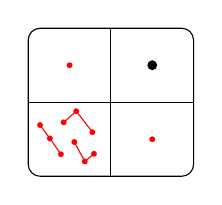
\begin{tikzpicture}[scale=0.5, every node/.style={scale=0.5}]
\def\xscale{1.0} % Horizontal scale factor
\def\yscale{1.0} % Vertical scale factor
\def\spnt{0.075} % Size of smaller points
\def\lpnt{0.125} % Size of larger points
\draw[rounded corners=2ex*0.5] (0,0) rectangle (4.2*\xscale,3.76*\yscale);
\draw (2.1*\xscale, 3.76*\yscale) -- (2.1*\xscale, 0);
\draw (0, 1.88*\yscale) -- (4.2*\xscale, 1.88*\yscale);
\fill[red] (1.05*\xscale, 2.82*\yscale) circle (\spnt);
\fill[red] (3.15*\xscale, 0.94*\yscale) circle (\spnt);
\fill[red] (0.9*\xscale, 1.37*\yscale) circle (\spnt);
\fill[red] (1.2199471753311761*\xscale, 1.6524363073940609*\yscale) circle (\spnt);
\fill[red] (1.63*\xscale, 1.12*\yscale) circle (\spnt);
\draw[red] (0.9*\xscale, 1.37*\yscale) -- (1.2199471753311761*\xscale,1.6524363073940609*\yscale) -- (1.63*\xscale,1.12*\yscale);
\fill[red] (1.17*\xscale, 0.87*\yscale) circle (\spnt);
\fill[red] (1.436829177631258*\xscale, 0.37686266458866924*\yscale) circle (\spnt);
\fill[red] (1.67*\xscale, 0.57*\yscale) circle (\spnt);
\draw[red] (1.17*\xscale, 0.87*\yscale) -- (1.436829177631258*\xscale,0.37686266458866924*\yscale) -- (1.67*\xscale,0.57*\yscale);
\fill[red] (0.3*\xscale, 1.3*\yscale) circle (\spnt);
\fill[red] (0.55*\xscale, 0.96*\yscale) circle (\spnt);
\fill[red] (0.83*\xscale, 0.56*\yscale) circle (\spnt);
\draw[red] (0.3*\xscale, 1.3*\yscale) -- (0.55*\xscale,0.96*\yscale) -- (0.83*\xscale,0.56*\yscale);
\fill (3.150000000000005*\xscale,2.8210223642172525*\yscale) circle (\lpnt);
\end{tikzpicture}
}
\newcommand{\tfour}{%
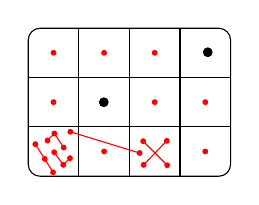
\begin{tikzpicture}[scale=0.5, every node/.style={scale=0.5}]
\def\xscale{1.0} % Horizontal scale factor
\def\yscale{1.0} % Vertical scale factor
\def\spnt{0.075} % Size of smaller points
\def\lpnt{0.125} % Size of larger points
\draw[rounded corners=2ex*0.5] (0,0) rectangle (5.14*\xscale,3.76*\yscale);
\draw (1.285*\xscale, 3.76*\yscale) -- (1.285*\xscale, 0);
\draw (2.57*\xscale, 3.76*\yscale) -- (2.57*\xscale, 0);
\draw (3.855*\xscale, 3.76*\yscale) -- (3.855*\xscale, 0);
\draw (0, 1.2533333333333332*\yscale) -- (5.14*\xscale, 1.2533333333333332*\yscale);
\draw (0, 2.5066666666666664*\yscale) -- (5.14*\xscale, 2.5066666666666664*\yscale);
\fill[red] ({(0*1.285+0.6425)*\xscale}, {(1*1.253+0.63)*\yscale}) circle (\spnt);
\fill[red] ({(0*1.285+0.6425)*\xscale}, {(2*1.253+0.63)*\yscale}) circle (\spnt);
\fill[red] ({(1*1.285+0.6425)*\xscale}, {(0*1.253+0.63)*\yscale}) circle (\spnt);
\fill[red] ({(1*1.285+0.6425)*\xscale}, {(2*1.253+0.63)*\yscale}) circle (\spnt);
\fill[red] ({(2*1.285+0.6425)*\xscale}, {(1*1.253+0.63)*\yscale}) circle (\spnt);
\fill[red] ({(2*1.285+0.6425)*\xscale}, {(2*1.253+0.63)*\yscale}) circle (\spnt);
\fill[red] ({(3*1.285+0.6425)*\xscale}, {(0*1.253+0.63)*\yscale}) circle (\spnt);
\fill[red] ({(3*1.285+0.6425)*\xscale}, {(1*1.253+0.63)*\yscale}) circle (\spnt);
\fill[red] (2.93*\xscale, 0.29*\yscale) circle (\spnt);
\fill[red] (3.52*\xscale, 0.9*\yscale) circle (\spnt);
\draw[red] (2.93*\xscale, 0.29*\yscale) -- (3.52*\xscale,0.9*\yscale);
\fill[red] (1.07*\xscale, 1.13*\yscale) circle (\spnt);
\fill[red] (2.83*\xscale, 0.59*\yscale) circle (\spnt);
\draw[red] (1.07*\xscale, 1.13*\yscale) -- (2.83*\xscale,0.59*\yscale);
\fill[red] (2.92*\xscale, 0.89*\yscale) circle (\spnt);
\fill[red] (3.53*\xscale, 0.28*\yscale) circle (\spnt);
\draw[red] (2.92*\xscale, 0.89*\yscale) -- (3.53*\xscale,0.28*\yscale);
\fill[red] (0.49*\xscale, 0.91*\yscale) circle (\spnt);
\fill[red] (0.6644210751853692*\xscale, 1.086774200246225*\yscale) circle (\spnt);
\fill[red] (0.9*\xscale, 0.73*\yscale) circle (\spnt);
\draw[red] (0.49*\xscale, 0.91*\yscale) -- (0.6644210751853692*\xscale,1.086774200246225*\yscale) -- (0.9*\xscale,0.73*\yscale);
\fill[red] (0.66*\xscale, 0.61*\yscale) circle (\spnt);
\fill[red] (0.89*\xscale, 0.29*\yscale) circle (\spnt);
\fill[red] (1.06*\xscale, 0.46*\yscale) circle (\spnt);
\draw[red] (0.66*\xscale, 0.61*\yscale) -- (0.89*\xscale,0.29*\yscale) -- (1.06*\xscale,0.46*\yscale);
\fill[red] (0.18033887520734232*\xscale, 0.816133743581277*\yscale) circle (\spnt);
\fill[red] (0.42*\xscale, 0.44*\yscale) circle (\spnt);
\fill[red] (0.63*\xscale, 0.1*\yscale) circle (\spnt);
\draw[red] (0.18033887520734232*\xscale, 0.816133743581277*\yscale) -- (0.42*\xscale,0.44*\yscale) -- (0.63*\xscale,0.1*\yscale);
\fill (1.92*\xscale,1.88*\yscale) circle (\lpnt);
\fill (4.56*\xscale,3.15*\yscale) circle (\lpnt);
\end{tikzpicture}
}
\newcommand{\tpair}{%
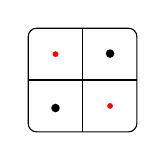
\begin{tikzpicture}[scale=0.35, every node/.style={scale=0.35}, baseline=(current bounding box.center)]
\def\xscale{1.0} % Horizontal scale factor
\def\yscale{1.0} % Vertical scale factor
\def\spnt{0.105} % Size of smaller points
\def\lpnt{0.155} % Size of larger points
\draw[rounded corners=2ex*.35] (0,0) rectangle (3.94*\xscale,3.76*\yscale);
\draw (1.97*\xscale, 3.76*\yscale) -- (1.97*\xscale, 0);
\draw (0, 1.88*\yscale) -- (3.94*\xscale, 1.88*\yscale);
\fill (0.99*\xscale,0.864920127795527*\yscale) circle (\lpnt);
\fill (2.97*\xscale,2.841054313099042*\yscale) circle (\lpnt);
\fill[red] (0.99*\xscale,3.76*0.75*\yscale) circle (\spnt);
\fill[red] (3*0.99*\xscale,3.76*0.25*\yscale) circle (\spnt);
\end{tikzpicture}
}
    \begin{center}
    \begin{tikzpicture}[scale=0.8, every node/.style={scale=0.8}]
        \node (root) at (0, 0) {\wordclass{8}{$(\varepsilon,\set{0,1},\set{11})$}};
        \node (lvl_1_1) at (-4, -2.25) {\wordclass{8}{$(0,\set{0,1},\set{11})$}};
        \node (lvl_1_2) at (0, -2.25) {\wordclass{8}{$\set{\varepsilon}$}};
        \node (lvl_1_3) at (4, -2.25) {\wordclass{8}{$(1,\set{0,1},\set{11})$}};
        \node (lvl_2_1) at (-6, -4.5) {\wordclass{8}{$\set{0}$}};
        \node (lvl_2_2) at (-2, -4.5) {\wordclass{8}{$(\varepsilon,\set{0,1},\set{11})$}};
        \node (lvl_2_3) at (1, -4.5) {\wordclass{8}{$\set{1}$}};
        \node (lvl_2_4) at (4, -4.5) {\wordclass{8.5}{$(10,\set{0,1},\set{11})$}};
        \node (lvl_2_5) at (7, -4.5) {\wordclass{8.5}{$(11,\set{0,1},\set{11})$}};
        \node (lvl_3_1) at (2, -6.75) {\wordclass{8}{$\set{10}$}};
        \node (lvl_3_2) at (6, -6.75) {\wordclass{8.5}{$(\varepsilon,\set{0,1},\set{11})$}};
        \node (lvl_4_1) at (0, -9) {\wordclass{8}{$\set{1}$}};
        \node (lvl_4_2) at (4, -9) {\wordclass{8}{$\set{0}$}};
        \ptedge{(root)}{(-0.5,1.2)}{(lvl_1_1)}{(-0.5,1.3)}
        \ptedge{(root)}{(-0.5,1.2)}{(lvl_1_2)}{(-0.5,1.3)}
        \ptedge{(root)}{(-0.5,1.2)}{(lvl_1_3)}{(-0.5,1.3)}
        \ptedge{(lvl_1_1)}{(-0.5,1.2)}{(lvl_2_1)}{(-0.5,1.3)}
        \ptedge{(lvl_1_1)}{(-0.5,1.2)}{(lvl_2_2)}{(-0.5,1.3)}
        \ptedge{(lvl_1_3)}{(-0.5,1.2)}{(lvl_2_3)}{(-0.5,1.3)}
        \ptedge{(lvl_1_3)}{(-0.5,1.2)}{(lvl_2_4)}{(-0.5,1.3)}
        \ptedge{(lvl_1_3)}{(-0.5,1.2)}{(lvl_2_5)}{(-0.5,1.3)}
        \ptedge{(lvl_2_4)}{(-0.5,1.2)}{(lvl_3_1)}{(-0.5,1.3)}
        \ptedge{(lvl_2_4)}{(-0.5,1.2)}{(lvl_3_2)}{(-0.5,1.3)}
        \ptedge{(lvl_3_1)}{(-0.5,1.2)}{(lvl_4_1)}{(-0.5,1.3)}
        \ptedge{(lvl_3_1)}{(-0.5,1.2)}{(lvl_4_2)}{(-0.5,1.3)}
    \end{tikzpicture}
    \end{center}
    \begin{center}
    \begin{tikzpicture}
        \node (root) at (-0.5, 0) {\tone};
        \node (lvl_1_1) at (-3,-2.25) {\ttwo};
        \node (lvl_1_2) at (0,-2.25) {\tnodeempty};
        \node (lvl_1_3) at (3,-2.25) {\tthree};
        
        \node (lvl_2_1) at (-4.5,-5.5) {\tone};
        \node (lvl_2_2) at (-2, -5.5) {\todesingle{\point{0.08}}};
        
        \node (lvl_2_3) at (1.75,-5.5) {\tfour};
        \node (lvl_2_4) at (4.25,-5.5) {\todesingle{\point{0.08}}};
        
        \node (lvl_3_1) at (0,-9) {\tone};
        \node (lvl_3_2) at (3.25,-8.73) {\tpair};
        
        \node (lvl_4_1) at (2,-11.75) {\todesingle{\point{0.08}}};
        \node (lvl_4_2) at (4.5,-11.75) {\todesingle{\point{0.08}}};
        
        \ptedge{(root)}{(0,1.2)}{(lvl_1_1)}{(-0.5,1.3)}
        \ptedge{(root)}{(0,1.2)}{(lvl_1_2)}{(-0.5,1.3)}
        \ptedge{(root)}{(0,1.2)}{(lvl_1_3)}{(-0.5,1.3)}
        
        \ptedge{(lvl_1_1)}{(-0.5,0.25)}{(lvl_2_1)}{(0,1.3)}
        \ptedge{(lvl_1_1)}{(-0.5,0.25)}{(lvl_2_2)}{(-0.5,1.3)}
        \ptedge{(lvl_1_3)}{(-0.5,0.25)}{(lvl_2_3)}{(-0.5,1.3)}
        \ptedge{(lvl_1_3)}{(-0.5,0.25)}{(lvl_2_4)}{(-0.5,1.3)}
        
        \ptedge{(lvl_2_3)}{(-0.5,0.25)}{(lvl_3_1)}{(0,1.3)}
        \ptedge{(lvl_2_3)}{(-0.5,0.25)}{(lvl_3_2)}{(-0.5,1.02)}
        
        
        \ptedge{(lvl_3_2)}{(-0.5,0.53)}{(lvl_4_1)}{(-0.5,1.3)}
        \ptedge{(lvl_3_2)}{(-0.5,0.53)}{(lvl_4_2)}{(-0.5,1.3)}
        
    \end{tikzpicture}
    \end{center}
}
    \caption{The grammar of the two specifications found by the bijection finder for binary strings avoiding two consecutive ones and $\Av{231,312,321}$.}
    \label{fig:fibwordpermtrees}
\end{figure}

\section{Permutation classes}
